\section{Distribution of prominence in an online labor market}
\label{sec:expr}

In this section we show that conventional approaches to ordering
platform participants---statically ranking individuals based on some
semi-permanent measure of relevancy, which we call assortive
ranking---leads to radically unequal allocations of prominence. We do
this using data from oDesk, a large online labor market. After
illustrating the problem, we evaluate the algorithms presented earlier
(EP and RT) through a series of simulations. We compare the algorithms
in terms of running time and performance to determine whether they can
be used in practice. We also assess how far RT deviates from the
exact proportion criterion, which is only guaranteed by EP.

\subsection{Prominence allocation in a labor marketplace}
\label{sec:expr-odesk}

In this section we use data from the oDesk
marketplace\footnote{http://www.odesk.com} to study how the prominence
in search results reflects the merit of the individuals that
participate in the results. oDesk is an online labor marketplace that
provides employers of two different ways to find prospective
contractors:
\begin{enumerate}
\item Employers can leverage a search interface that allows them to
  retrieve contractor profiles that are relevant to some
  keyword. Employers have the option to send an interview invitation
  to any of the retrieved contractors.
\item Employers may also wait for contractors to apply after they have
  posted a job. When a contractor applies to a job, the associated
  employer is notified via email. The employer reviews the contractor
  profile and the application cover letter and decides whether to
  invite the contractor to interview for the job.
\end{enumerate}

The two alternative ways to reach contractors allow us to obtain
contractor prominence and merit estimates. In case of search, the way
that oDesk ranks contractors makes them more or less visible to the
employers. Thus, the profile views that the contractors receive
through clicks on the search results are indicative of the prominence
that oDesk provides them. In case of job applications, the email
notification and the typically small number of applicants per job
(around 10 applicants) makes it exceeedingly likely that the employer
will view each of the applications and the corresponding
profiles. Given that an employer views a profile, the probability of
an interview invitation or the probability of hiring is indicative of
the contractor's merit.

%Zipf-Mandelbrot LNRE model.
%Parameters:
%   Shape:          alpha = 0.2884794 
%   Upper cutoff:       B = 8.565862e-05 
% [ Normalization:      C = 557.3199 ]
%Population size: S = Inf 
%Sampling method: Poisson, with exact calculations.
%
%Parameters estimated from sample of size N = 10465514:
%                  V       V1       V2       V3       V4      V5    
%   Observed: 233215 66207.00 19856.00 13163.00 10823.00 8839.00 ...
%   Expected: 233215 75584.19 26889.86 15340.85 10399.26 7719.41 ...
%
%Goodness-of-fit (multivariate chi-squared test):
%         X2 df p
%   59884.04 14 0
\begin{figure}[t]
  \includegraphics[width=0.5\columnwidth]{../simulations/results/click_distribution.png}
  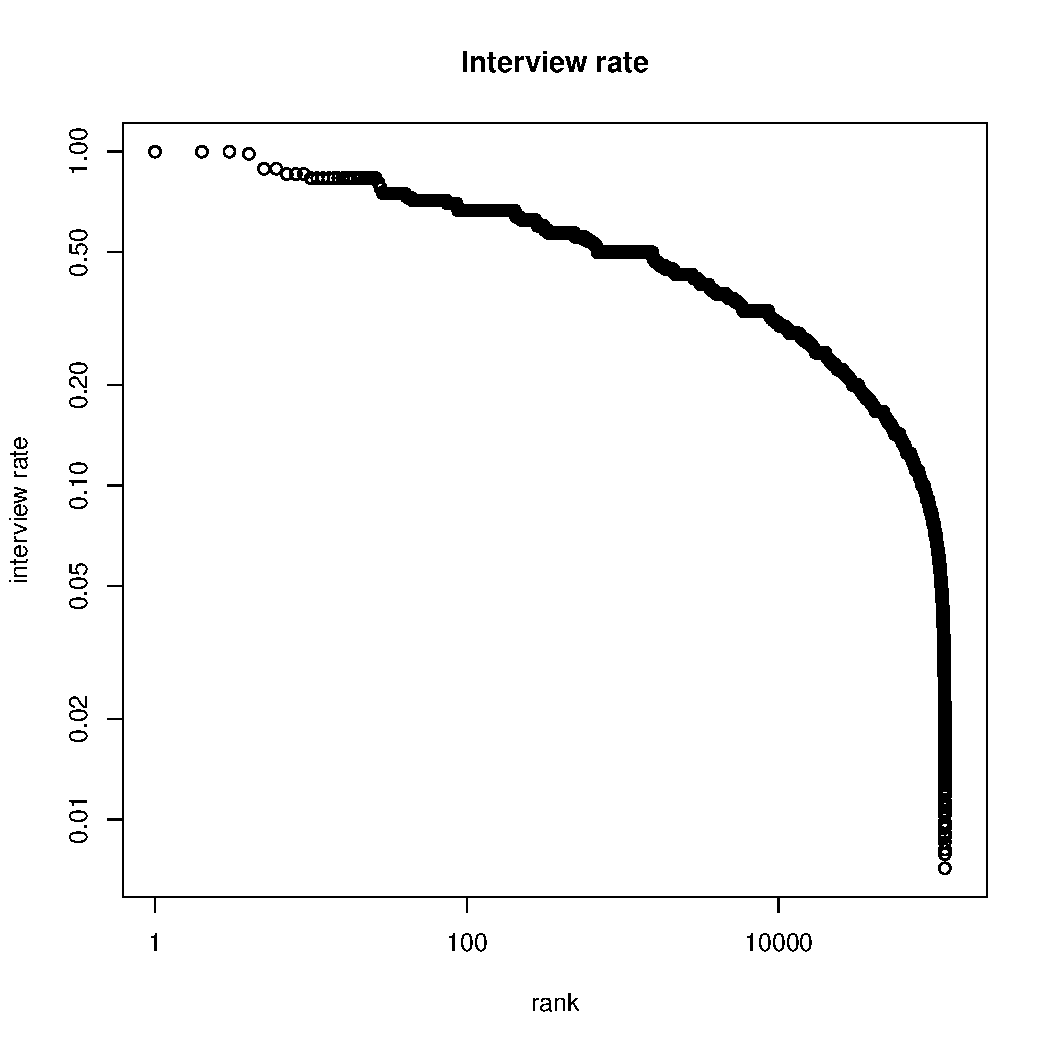
\includegraphics[width=0.5\columnwidth]{../simulations/results/interviewrate_distribution.png}
  \caption{(a) Click distribution per rank position in oDesk
    contractor search. (left) (b) Interview rate at oDesk over a
    period of eight months. (right)}
  \label{fig:clicks}
\end{figure}
To estimate the prominence we use the oDesk contractor search logs
over the period of two weeks of January. The log contains a record for
every click on the search results and each record shows the position
in search and the target contractor profile. In
Figure~\ref{fig:clicks}(a) we plot the click distribution per search
rank position in oDesk contractor search in double logarithmic
scale. The number of clicks drops from approximately 60K in the first
position to 15K in the second and around 200 in the tenth position
(the last position of the first results page). We fitted a Zipfian
distribution to the data and the estimated exponent is 1.35. Our
results are similar to click distribution in traditional web search
\cite{ali2007robust} and indicate dramatic decrease in prominence even
for consecutive positions in search results. In the next paragraph we
show that such distribution is not justified by the contractor merit
distribution.

%\begin{figure}[t]
%  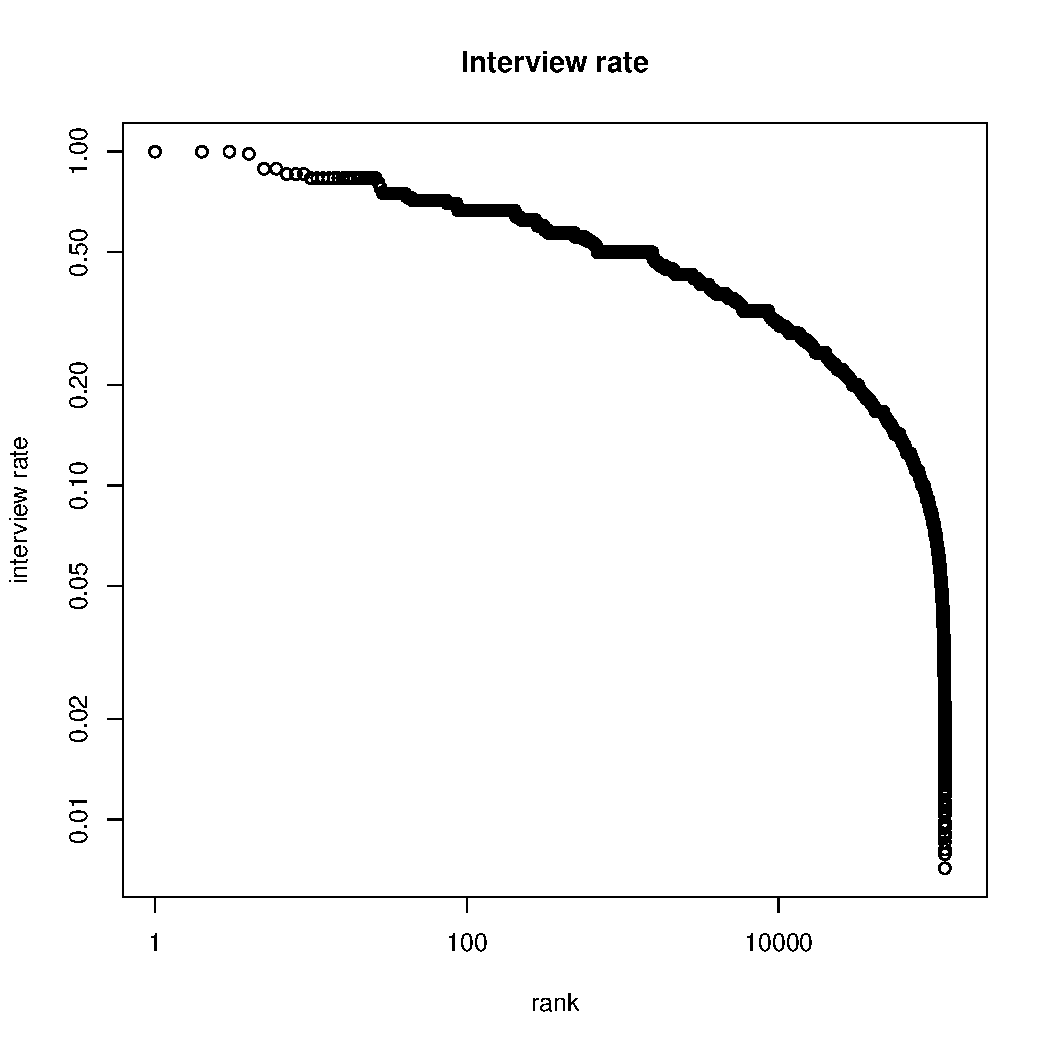
\includegraphics[width=0.4\columnwidth]{../simulations/results/interviewrate_distribution.png}
%  \caption{Interview rate at oDesk over a period of eight months.}
%  \label{fig:interviewrate}
%\end{figure} 

Any constructed measure of merit will be somewhat arbitrary and highly
platform dependent. For oDesk, a reasonable measure of merit is a
constractor's ``success rate'' in seeking jobs. We looked at the job
application history at oDesk over a period of eight months (June 2011
through January 2012) and we calculated each contractor's interview
rate, defined as the ratio of his job applications that evolved into
an interview over his or her total job applications in the period. In
Figure~\ref{fig:clicks}(b) we plot the interview rate distribution in
double logarithmic scale.

By comparing the two Figures~\ref{fig:clicks}(a),(b) we can see how
the search ranking imposes an artificial boost on prominence that is
not justified from an individual's merit.  The gap between the two
distrcibutions shows that there are many contractors who have almost
equal success in convincing with their job applications employers to
setup an interview but receive different prominence through the search
interface.


